% Name: Donut chart
% Description: Hours on a project by phase as a ring whose four parts add up to 100%, with the total in the middle and a legend beside it.
% Tags: donut chart, ring chart, percentages, proportions

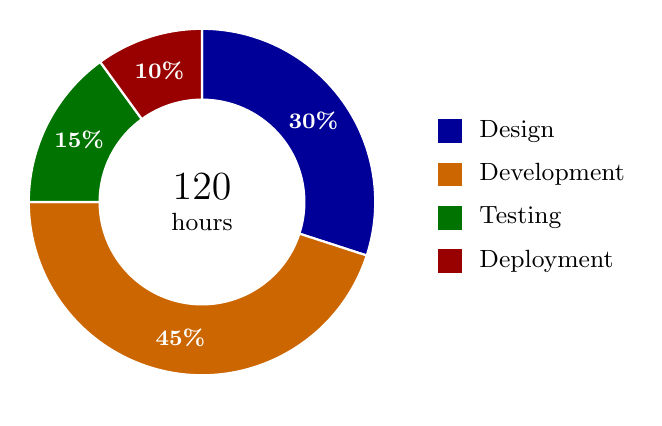
\begin{tikzpicture}[font=\small]
  % 120 hours: design 36 (30%), development 54 (45%), testing 18 (15%), and deployment 12 (10%).
  \foreach \p/\name/\c [remember=\b as \a (initially 0), evaluate=\p as \b using \a+\p, count=\i] in
    {30/Design/blue!60!black, 45/Development/orange!80!black, 15/Testing/green!45!black, 10/Deployment/red!60!black} {
    \fill[\c, draw=white, thick] (90-3.6*\a:2.2) arc[start angle=90-3.6*\a, end angle=90-3.6*\b, radius=2.2]
      -- (90-3.6*\b:1.3) arc[start angle=90-3.6*\b, end angle=90-3.6*\a, radius=1.3] -- cycle;
    \pgfmathsetmacro\mid{90 - 1.8*(\a + \b)}
    \node[white, font=\footnotesize\bfseries] at (\mid:1.75) {\p\%};
    \fill[\c] (3,1.3-0.55*\i) rectangle ++(0.3,0.3);
    \node[anchor=west] at (3.4,1.45-0.55*\i) {\name};
  }
  \node[align=center] at (0,0) {\Large 120\\hours};
\end{tikzpicture}
